\documentclass{standalone}

\usepackage[rgb]{xcolor}
\usepackage{tikz}
\usepackage{fix-cm}
\usepackage{shadowtext}

\usetikzlibrary{shadows.blur}
\usetikzlibrary{shapes.symbols}

\newdimen\pinA
\newdimen\pinB
\newdimen\pinC

\setlength{\pinA}{14mm}
\setlength{\pinB}{17mm}
\setlength{\pinC}{25mm}

\definecolor{pin}{gray}{0}
\definecolor{texred}{HTML}{E01C24}

\begin{document}
  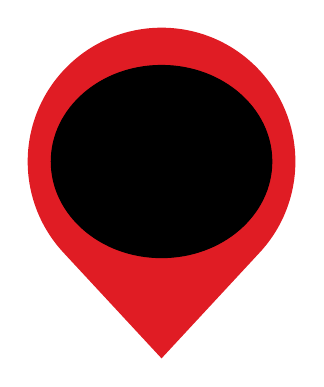
\begin{tikzpicture}
    \useasboundingbox (-\pinB, -\pinC) (\pinB, \pinB);
    \pgfmathsetmacro{\pinAngle}{acos(\pinB/\pinC)}%
    \pgfmathsetmacro{\pinAngleRight}{270+\pinAngle}%
    \path[fill=pin, color=texred, even odd rule,
      %blur shadow={shadow blur steps=5}
    ]
      (\pinAngleRight:\pinB)
      arc[
        at={(0,0)},
        start angle=\pinAngleRight,
        delta angle=360-2*\pinAngle,
        radius=\pinB,
      ]
       -- (0, -\pinC);
      \filldraw circle [at={(0,0)}, x radius=\pinA, y radius=-1.8mm+\pinA];
      \node at (0,-0.1) {\fontsize{40}{46}\selectfont\TeX};
  \end{tikzpicture}
\end{document}
